\documentclass[reprint,amsmath,amssymb,aps,twoside]{revtex4-2} % for editor use only

% For initial submission use these lines
%\documentclass[amsmath,amssymb,aps,endfloats,linenumbers]{revtex4-2}



% DO NOT CHANGE THINGS BELOW HERE
\usepackage{graphicx}
\usepackage{amsmath,amssymb,amsfonts}
\usepackage{dcolumn}
\usepackage{bm}
\usepackage{siunitx}
%\usepackage{tikz,pgfplots}
\sisetup{separate-uncertainty=true, multi-part-units=single}
\usepackage[colorlinks,allcolors=blue]{hyperref}
\usepackage{cleveref}
\crefname{equation}{}{}
\crefname{figure}{Fig.}{Figs.}
\crefname{table}{Table}{Tables}
\usepackage{svg}
\svgpath{{./figures}}
\makeatletter
\def\blfootnote{\xdef\@thefnmark{}\@footnotetext}
\makeatother




% set PDF metadata
% AUTHORS EDIT THIS PART
\hypersetup{%
pdftitle={Testing energy conservation through popper launch and compression experiments}, % full title here
pdfauthor={David Pevzner, Joe C Cardillo, Ashmaan Siddiqui, Jake Croft, Justin J Chan, and Bobby Kapoor}, % full author list here
}


\usepackage{fancyhdr}
\pagestyle{fancy}
\fancyhf{}
\fancyhead[RE,RO]{J S\&E \textbf{2}, 106--109 (2026)} % FOR EDITOR ONLY
\fancyhead[LO]{Pevzner \emph{et al}} % if many authors
\fancyhead[LE]{Testing energy conservation through popper launch and compression experiments} 
\fancyfoot[C]{\thepage}
\fancypagestyle{mytitlepage}{
\fancyhf{}
\fancyhead[C]{Journal of Science \& Engineering \textbf{2}, 106--109 (2026)} % FOR EDITOR ONLY
\fancyfoot[C]{\thepage}
%\fancyfoot[L]{\scriptsize\copyright\ 2026 Journal of Science \& Engineering, \href{https://creativecommons.org/licenses/by-nc/4.0/}{CC-BY-NC 4.0}}
\fancyfoot[L]{\scriptsize\copyright\ 2026 J S\&E \href{https://creativecommons.org/licenses/by-nc/4.0/}{CC-BY-NC 4.0}}
}


\begin{document}
\setcounter{page}{106} % FOR EDITOR USE ONLY
%\linenumbers % FOR EDITOR USE ONLY

% AUTHORS EDIT THIS PART
\title{Testing energy conservation through popper launch and compression experiments}
\author{David Pevzner}
\email[Contact author: ]{427dpevzner@frhsd.com} % use FRHSD address
\author{Joe C Cardillo}
\author{Ashmaan Siddiqui}
\author{Jake Croft}
\author{Justin J Chan}
\author{Bobby Kapoor}
% For S&E authors
\affiliation{Science \& Engineering Magnet Program, \href{https://manalapan.frhsd.com/}{Manalapan High School}, Englishtown, NJ 07726 USA}
%\date{\today}
\received{30 January 2026}
\accepted[accepted~]{31 March 2026}
\published[published~]{17 May 2026}


\begin{abstract}
The principle of energy conservation predicts that energy is never lost; it only changes forms. To test this principle experimentally, we launched popper toys that, when compressed, store elastic potential energy, which is converted into kinetic energy and gravitational potential energy as the popper launches. We also compressed the popper to determine the total elastic potential energy stored in it before launch. Ultimately, by comparing the kinetic and potential energies at different stages of the launch and assuming negligible air resistance, we found convincing evidence that mechanical energy is not constant; however, this does not imply that energy is not conserved, considering we failed to account for air resistance. 

\vspace{1em} % Add space before DOI
\noindent DOI: \href{https://doi.org/10.64804/q69tgd65}{10.64808/q69tgd65}
\end{abstract}

\keywords{popper, launch, elastic potential energy, energy conservation}

\maketitle\thispagestyle{mytitlepage}
\blfootnote{\\\emph{Published by the Journal of Science \& Engineering under the terms of the \href{https://creativecommons.org/licenses/by-nc/4.0/}{Creative Commons Attribution-NonCommercial 4.0 International} license. Further distribution of this work must maintain attribution to the author(s) and the published article's title, journal citation, and DOI.}}

%The current column width is \the\columnwidth

\section{Introduction}
Kinetic energy is the energy associated with the motion of an object and represents the work done to speed up an object to a certain velocity. It is a scalar quantity that increases with both mass and velocity and is given by \cite{tipler,barrons,openstax}:
\begin{equation}
\text{KE} = \frac{1}{2}mv^2.
\label{eq:1}
\end{equation}

Potential energy is the energy associated with the position of an object. Each conservative(i.e. path-independent) force gives rise to a different form of potential energy, but in general, the change in potential energy of conservative forces is given by the following integral \cite{tipler,barrons,openstax}:
\begin{equation}
\Delta \text{PE} = -\int\vec{F}\cdot d \vec{x}.
\label{eq:2}
\end{equation}

Note that this implies that we can find the area under the curve of the graph of $F$ vs $x$ and use this to find total potential energy. Considering \cref{eq:2} with $F$ being given by the force of gravity, which is $mg$ in the negative direction, with $g=\qty{9.8}{\meter\per\second\squared}$, we find gravitational potential energy at $h$ to be given by \cite{tipler,barrons,openstax}:
\begin{equation}
\text{PE} - 0 = -\int_0^h -mg dy. 
\label{eq:3}
\end{equation}
Using the reverse power rule, we find the indefinite integral and find the difference of it evaluated at the upper and lower bounds as follows \cite{tipler,barrons,openstax}:
\begin{equation}
\text{PE} = mgy \bigg|^h_0 = mgh.
\label{eq:4}
\end{equation}
The sum of the total kinetic and potential energies of a system is known as mechanical energy. According to the principle of energy conservation, in the absence of non-conservative forces such as drag and friction, mechanical energy within a system remains constant. 

In an effort to test the accuracy of this principle, we launched poppers and observed whether energy was conserved as elastic potential energy is converted into kinetic energy, which becomes gravitational potential energy. That is, we tested to see if the kinetic energy of the poppers right after launch ($\text{KE}_0$) was equal to the gravitational potential energy when the poppers reached their maximum height ($\text{GPE}_f$). Our null hypothesis and alternative hypothesis were:
\begin{align}
H_0 : \text{KE}_0 &= \text{GPE}_f, \\
H_a : \text{KE}_0 &\neq \text{GPE}_f.
\end{align}

We also analyzed the mechanical work done in compressing the poppers, in order to determine the total energy stored in the form of elastic potential energy prior to launch:
\begin{equation}
W = \int \vec{F} \cdot d\vec{x}.
\label{eq:5}
\end{equation} 
The work done, and the elastic potential energy prior to launch, should also be equal in magnitude to the kinetic energy at launch in an ideal system. In a real system, however, friction and other nonconservative forces are expected to dissipate some portion of the energy, resulting in $\text{KE}_0 < W$. Computing $W$ allows us to examine if energy loss is occurring primarily during the launch process, i.e. $W > \text{KE}_0$, or if energy loss is dominated by in-flight mechanisms like friction, i.e. $\text{KE}_0>\text{GPE}_f$. 







\section{Methods and materials}
In our experiment, we utilized a \qty{5.7}{\gram} crying emoji popper toy (``Jumping Gens''; Liberty Imports; Allentown, PA) made of a ethylene vinyl acetate (EVA) foam head and body (i.e. coefficient of restitution $COR = \numrange{0.7}{0.95}$)\cite{simeonov:2016:coefficient}. 

\subsection{$\text{KE}_0$ and $\text{GPE}_f$ measurements}
Popper launch kinematics were recorded using a Smartphone (S25; Samsung; Suwon, South Korea) operated at \qty{120}{frame\per\second}. To provide scale calibration, we placed two metersticks in the frame and used a bubble level to ensure the metersticks were aligned vertically. 

To measure the velocity of the popper at launch, we recorded the launch frame by frame and calculated the velocity of the popper by multiplying the frame rate by the distance traveled between a single frame. Note that we measure the velocity over as short a time period as possible to reduce error due to gravitational acceleration. We then used \cref{eq:1} to calculate the kinetic energy of the popper based on its initial velocity ($\text{KE}_0$). We also measured the maximum height reached by the poppers using the video recordings. We then used \cref{eq:4} to calculate the gravitational potential energy at the maximum height ($\text{GPE}_f$). The various stages of the launch of the popper as well as our experimental setup is show in \cref{fig:1} and the data collected from our launches is shown in \cref{tab:1}. We then applied a $t$-test to see if the difference $\text{KE}_0-\text{GPE}_f$ was significantly different from zero \cite{starnes:2015:practice,R,ggplot2,dplyr}. 
\begin{figure}
\begin{center}
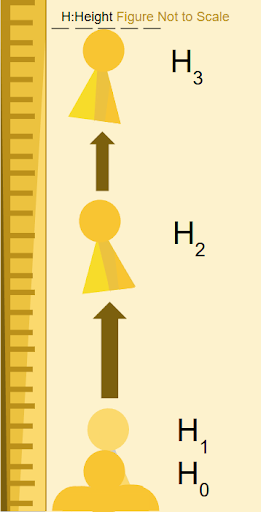
\includegraphics[width=0.5\columnwidth]{figures/launch.png}
\end{center}
\caption{Popper launch mechanism.}
\label{fig:1}
\end{figure}

\subsection{$W$ measurement}
To measure the mechanical work done in compressing the popper, we placed the popper on top of a digital scale (Arboleaf CK10I; Plano, TX) to measure force, as seen in \cref{fig:1b}. We used a scissor jack (\qtyproduct{8x8}{inch} area, min height \qty{3}{inch}) with ruler clamped to a ringstand for distance measurements. We zeroed the scale and the ruler at the point where the scissor jack was just touching the head of the popper. We then lowered the scissor jack in increments of \qty{0.005}{\meter}. Scale readings were converted to \unit{\newton} using $F=mg$. We conducted two replicates from unloaded to fully compressed. \Cref{eq:5} was used to find the mechanical work done in compressing the popper. The area under the resulting curve was numerically integrated using the trapezoid method \cite{calculus,R}. 
\begin{figure}
\begin{center}
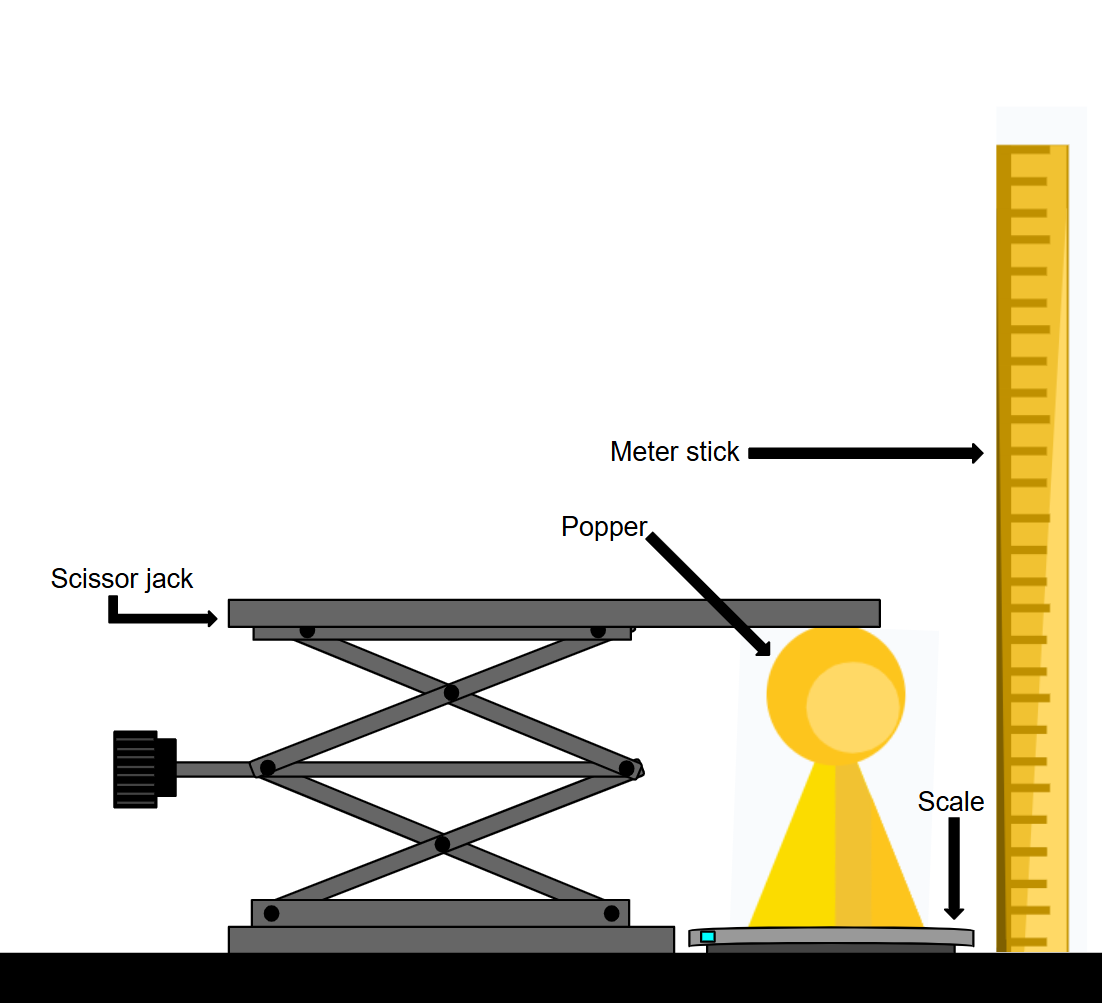
\includegraphics[width=0.75\columnwidth]{figures/compress.png}
\end{center}
\caption{Scissor jack setup}
\label{fig:1b}
\end{figure}

Data and analysis code are available at \url{https://github.com/devangel77b/427jcardillo-lab3}.
    
    
    
    
\section{Results}
From this data set, we find the sample mean and sample standard deviation of the difference in kinetic and potential energy to be \qty{0.048}{\joule} and \qty{0.022}{\joule}, respectively. This gives a test statistic of 7.44, which gives a two-sided $p$-value of \num{1.29e-5}.
\begin{table}
  \caption{Observed kinetic and potential energy}
  \label{tab:1}
  \begin{center}
  \begin{ruledtabular}
    \begin{tabular}{SSSS}
      {trial} & {$\text{KE}_0$, \unit{\joule}} & {$\text{GPE}_f$, \unit{\joule}} & {$\text{KE}_0-\text{GPE}_f$, \unit{\joule}} \\
      \colrule \\
      1  & 0.103 & 0.076 & 0.027 \\
      2  & 0.080 & 0.075 & 0.005 \\
      3  & 0.120 & 0.081 & 0.039 \\
      4  & 0.113 & 0.078 & 0.035 \\
      5  & 0.138 & 0.083 & 0.055 \\
      6  & 0.113 & 0.084 & 0.030 \\
      7  & 0.136 & 0.076 & 0.060 \\
      8  & 0.138 & 0.081 & 0.057 \\
      9  & 0.158 & 0.083 & 0.075 \\
      10 & 0.120 & 0.077 & 0.043 \\
      11 & 0.174 & 0.092 & 0.082 \\
      12 & 0.148 & 0.078 & 0.070 \\
    \end{tabular}
  \end{ruledtabular}
\end{center}
\end{table}


\begin{table}
\caption{Elastic force versus displacement for poppers}
\label{tab:2}
  \begin{center}
    \begin{ruledtabular}
      \begin{tabular}{SS}
        {displacement $x$, \unit{\meter}} & {force $F$, \unit{\newton}} \\
        \colrule \\
        0.005 & 1.49 \\
        0.005 & 1.47 \\ 
        0.010 & 2.74 \\
        0.010 & 2.88 \\
        0.015 & 4.30 \\
        0.015 & 4.31 \\
        0.020 & 5.91 \\
        0.020 & 5.49 \\
        0.025 & 7.92 \\
        0.025 & 7.42 \\
        0.030 & 6.49 \\
        0.030 & 7.01 \\
        0.035 & 5.49 \\
        0.035 & 5.85 \\
      \end{tabular}
    \end{ruledtabular}
  \end{center}
\end{table}
    


\begin{figure}
\begin{center}
%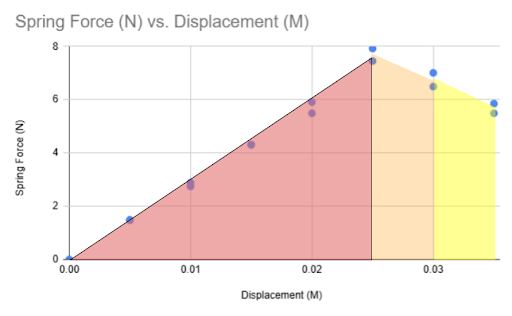
\includegraphics[width=\columnwidth]{figures/graph.png}
\includesvg[width=\columnwidth]{fig3}
\end{center}
\caption{Spring force (\unit{\newton}) vs. displacement (\unit{\meter}). The work done in compressing the popper is \qty{0.1573}{\joule}.}
\label{fig:2}
\end{figure}
Using the trapezoidal rule and averaging over points, we can calculate the work to compress the popper, and the energy stored within the spring to be \qty{0.1573}{\joule}.
%:
%%\begin{multline}
%%    W = U_\text{spring} = \int^{0.035}_0 F(x) dx = \frac{0.025(7.92+7.482)}{2}+\frac{0.005(7.92+7.482+6.49+7.012)}{2}+ \\ \frac{0.005(6.49+7.012+5.49+5.852)}{2}
%%\end{multline}
%\begin{multline}
%    W \approx \frac{0.025(7.92+7.482)}{2}+\frac{0.005(7.92+7.482+6.49+7.012)}{2}+ \\ \frac{0.005(6.49+7.012+5.49+5.852)}{2}
%\end{multline}





    
    
\section{Discussion}
\subsection{Energy loss mechanisms unaccounted for}
Our $p$-value of \num{1.29e-5}, which is far less than any reasonable significance level, leads us to reject our null hypothesis, suggesting that we have found convincing evidence that energy is not conserved when launching poppers. However, considering we did not account for the force of air resistance, this conclusion does not conclusively support that energy is not conserved. In fact, analyzing the data, it is clear that the potential energy was always less than the kinetic energy, which makes sense because energy was dissipated over time due to friction with air molecules. 

Our value for the elastic potential energy stored within the spring was greater than the initial kinetic energy with which the popper was launched for all the trials except for one, contradicting energy conservation, which would suggest the two forms of energy to be equal. This can be attributed to our use of an inconsistent human hand-based popper launch that does not fully compress the poppers. Moreover, if launches are not perfectly vertical, some of the popper's kinetic energy can go to the horizontal direction which we have no way of accounting for with our setup. In future experiments, a consistent and standardized way to compress the popper before launching is needed to address these issues.

\subsection{Inelastic energy loss}
Another source of error would be poppers holding less elastic energy over time due to repeated stretching and the gradual breakdown of their elastic material. When analyzing the spring force at different displacement values, we observed that the spring followed the linear nature of Hooke's law\cite{tipler} with $r^2 = 0.99$, 
\begin{equation}
F = kx
\end{equation}
However, at a displacement of approximately \qty{0.025}{\meter}, the graph deviated from Hooke’s law, with successive measured force values decreasing rather than increasing. We hypothesize that this occurred because the spring buckled at this displacement, causing it to no longer deform elastically and resulting in a significantly reduced measured force. This loss of elastic behavior can be interpreted in terms of the coefficient of restitution, a measure of how well a system returns energy when deformed. As the spring buckled, energy was dissipated through internal friction rather than stored elastically. 

\subsection{Air resistance}
To test if the magnitude of mechanical energy loss can be reasonably accounted for by air resistance, we performed a scaling calculation by calculating the work due to air resistance. To do this, we integrated the drag force
\begin{equation}
F = \frac{1}{2}\rho C_d Av^2
\end{equation}
with respect to $x$, applying the chain rule and reverse power rule, to find that 
\begin{align}
W_d 
&= \frac{1}{2}\rho C_d A\int v^2 dx, \\
&= \frac{1}{2}\rho C_d A\int_0^{\frac{v_0}{g}} v^2 \frac{dx}{dt} dt, \\
&\approx \frac{1}{2}\rho C_d A\int_0^{\frac{v_0}{g}} (v_0-gt)^3 dt, \\
&\approx \frac{\rho C_DAv_0^4}{8g}.
\end{align}
Note that we did not account for the air resistance's effect on the velocity in the integral, but this will not have a large affect on our results and is valid for or scaling/estimating purposes. Setting drag coefficient $C_d=1.0$, $\rho=\qty{1.225}{\kilo\gram\per\meter\cubed}$ for the density of air \cite{tipler}, $A=\qty{1e-3}{\meter\squared}$ for the cross sectional area of the popper, and $v_0=\qty{5.1}{\meter\per\second}$ (i.e. the minimum launch velocity we observed) as the initial velocity, we find that
\begin{equation}
W_d = \qty{0.011}{\joule}
\end{equation}
If we instead use the maximum launch velocity we observed (\qty{7.6}{\meter\per\second}), we find
\begin{equation}
W_d = \qty{0.052}{\joule}
\end{equation}
These two estimates bracket the energy differences in \cref{tab:1}, supporting the idea that the observed energy losses between $\text{KE}_0-\text{GPE}_f$ may be due to air resistance. 







    
    
\section{Acknowledgements}
JCC, JJC, JC, BK, AS, and DP collected the data. DP wrote the abstract, introduction, results, and part of the discussion. BK and AS wrote the Methods and Materials and created the figures. JCC wrote part of the discussion and labelled all figures. 







\bibliography{lab.bib}
\end{document}
